\section{Řídící jednotka}
% \textit{TODO: shrnutí funkce a požadavků -- komunikace s periferiemi, napajeni, wifi, status - led + display} 
Jedná se o jádro celého zařízení. Její funkcí je řízení celého systému a zároveň komunikace s uživatelem za pomoci Wi-Fi. Musí v sobě nést informaci o konfiguraci systému a na jejím základě zpracovávat data z jednotlivých připojených periferií. Podle uživatelem nastavených scénářů pak dynamicky reaguje na změny hodnot měřených akvaristických veličin a ovládá akční členy (osvětlení, ohřev, filtr vody). Za pomoci displaye a LED pásku také informuje uživatele o stavu zařízení. 

Řídící jednotka bude tvořena jednou speciálně navrženou DPS, které kromě samotného mikrokontroleru bude obsahovat také obvody ke snížení napájecího napětí externího zdroje na hodnotu \qty{5.2}{V} (odůvodnění v sekci~\ref{subsec:pocet-a-fce-vodicu-sbernice}). Toto napětí pak bude dále používáno pro napájení samotného mikrokontroleru řídící jednotky a zároveň vyvedeno na konektor pro připojení periferií. Blokové schéma na úrovni logických bloků v rámci jedné DPS je na obr.~\ref{fig:ridici-jednotka-blokove-schema}, jednotlivým částem se blíže věnují další sekce.

% \newlength{\schematicpdfoffset} % Definice nové délkové proměnné
\begin{figure}[h!]
    \centering
    % trim=left bottom right top
    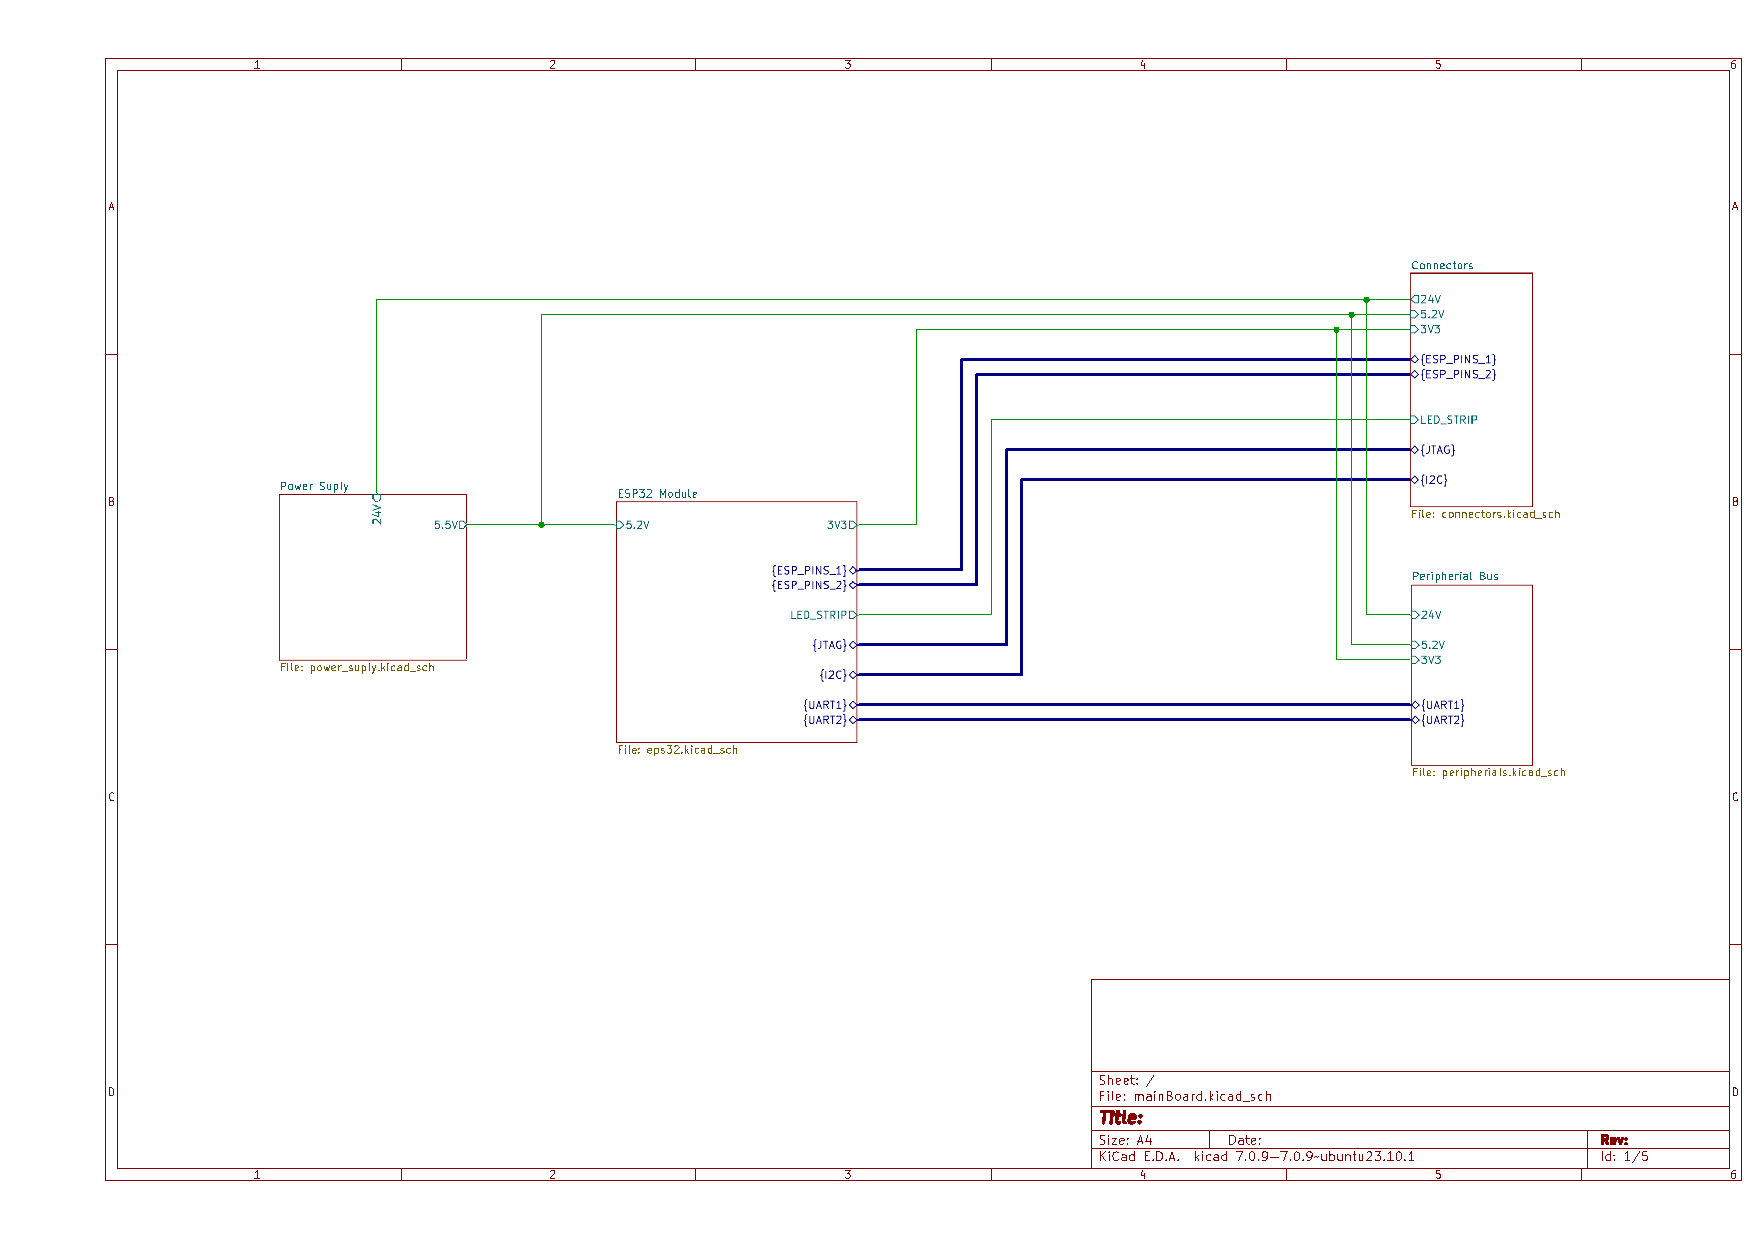
\includegraphics
    [
        width=\textwidth, 
        page=1, 
        trim=4.5cm 7.5cm 3cm 4cm, 
        clip
    ]{obrazky/exportovane/main-board-schematic.pdf}
    \caption{Blokové schéma řídící jednotky. Vytvořeno v KiCad 7.0.}
    \label{fig:ridici-jednotka-blokove-schema}
\end{figure}

    \subsection{MCU}
        % \textit{TODO: zdůvodnit výběr ESP32, informace o něm a schéma potřebných obvodů} 
        Při výběru vhodného mikrokontroleru bylo potřeba zohlednit výše zmíněné požadavky, tedy zejména Wi-Fi konektivita a dostatečný výkon k její obsluze, dvě volné UART periferie a dostatek GPIO pinů pro připojení zbylých modulů v hlavním šasi (viz obr.~\ref{fig:blokove-schema}). Na trhu existuje vícero výrobců nabízejících mikrokontrolery s vhodnými parametry, z důvodu jednoduchosti použití a nízké ceny byl nakonec zvolen model ESP32 od firmy Espressif, konkrétně modul WROOM-32E~\cite{esp32-wroom-32e-datasheet} s čipem ESP32-D0WDR2-V3~\cite{esp32-datasheet}. Tento mikrokontroler je často využíván v různých hobby projektech, ale také v komerčních aplikacích zejména v oblasti chytré domácnosti. Z tohoto důvodu k němu existuje velká škála softwarových knihoven a v rámci komunity uživatelů je také sdíleno mnoho projektů, kterými je možné se inspirovat.

        \subsection{Zapojení ESP32 modulu}
            Při tvorbě schématu bylo vycházeno z dokumentace výrobce~\cite{esp32-wroom-32e-datasheet} a také ze schématů různých vývojových desek. K zajištění správné a spolehlivé funkce modulu je potřeba dodržet několik věcí. Výřez schématu obsahující potřebné doplňující obvody je na obr.~\ref{fig:ridici-jednotka-esp-obvody}, schéma celé řídící jednotky se pak nachází v příloze (\textit{TODO reference} ). 

            \begin{figure}[h!]
                \centering
                % trim=left bottom right top
                \includegraphics
                [
                    width=0.9\textwidth, 
                    page=2, 
                    trim=2.5cm 6cm 15.5cm 1.5cm, 
                    clip
                ]{obrazky/exportovane/main-board-schematic.pdf}
                \caption{Podpůrné obvody pro modul ESP32-WROOM-E. Vytvořeno v KiCad 7.0.}
                \label{fig:ridici-jednotka-esp-obvody}
            \end{figure}

            Na napájecí pin (3V3) je třeba přivést stabilní napětí a opatřit ho blokovacími kondenzátory (C1, C3). Ke snížení napětí z původních \qty{5,2}{V} na požadovaných \qty{3,3}{V} je použit lineární regulátor TLV76133 (U4). 
            
            Dále je potřeba přivést kladné napětí na povolovací pin (EN), z dokumentace vyplývá, že by mělo být přivedeno až po ustálení napájecí linky. Uvedený časnutný ke stabilizaci je roven \(t_{STBL}=\qty{50}{\micro\second}\)~\cite{esp32-datasheet}. Požadované zpoždění zajistí RC článek (R1, C2) s časovou konstantou \(\tau\) : 
            \begin{equation}
                \tau=R_{1}C_{2}=\qty{10}{\kilo\ohm}\cdot \qty{1}{\micro\farad}=\qty{10}{\milli\second}
            \end{equation} 
            Jak je vidět, byla zvolena dostatečná návrhová rezerva. 

            Pro možnost resetu zařízení a nahrání nového firmware byly doplněny také dvě tlačítka (SW1, SW2)



    \subsection{Napájecí obvod}
        % \textit{TODO: schéma, výpočet hodnot součástek} 
        \begin{figure}[h!]
            \centering
            % trim=left bottom right top
            \includegraphics
            [
                width=0.9\textwidth, 
                page=3, 
                trim=5.5cm 4.5cm 4cm 2.5cm, 
                clip
            ]{obrazky/exportovane/main-board-schematic.pdf}
            \caption{Napájecí obvod řídící jednotky. Vytvořeno v KiCad 7.0.}
            \label{fig:ridici-jednotka-napajeni}
        \end{figure}

    \subsection{Ochrana konektorů}
        \textit{TODO: popsat principy ochrany, schéma} 